
\documentclass[10pt,a4paper]{article}
\usepackage[a4paper,margin=14mm,top=18mm,bottom=20mm,headheight=12pt,headsep=5mm,footskip=9mm]{geometry}
\usepackage{fontspec}
\usepackage{xcolor}
\usepackage{graphicx}
\usepackage{tikz}
\usepackage{tabularx}
\usepackage{array}
\usepackage{fancyhdr}
\usepackage{needspace}
\usepackage{multicol}
\usepackage{enumitem}
\defaultfontfeatures{Ligatures=NoCommon}
\IfFontExistsTF{Noto Sans CJK SC}{\setmainfont{Noto Sans CJK SC}\setsansfont{Noto Sans CJK SC}}{\setmainfont{DejaVu Sans}\setsansfont{DejaVu Sans}}
\IfFontExistsTF{DejaVu Sans}{\newfontfamily\BOQuoteFont{DejaVu Sans}}{\newfontfamily\BOQuoteFont{Latin Modern Sans}}
\newcommand{\BOApos}{{\BOQuoteFont\char"0027}}
\definecolor{BOBlue}{HTML}{0E6B72}
\definecolor{BOBright}{HTML}{20A66A}
\definecolor{BOGreen}{HTML}{00A651}
\definecolor{BONavy}{HTML}{1B2A34}
\definecolor{BOText}{HTML}{24323A}
\definecolor{BOMuted}{HTML}{7C878E}
\definecolor{BOLine}{HTML}{D9E1E6}
\definecolor{BOLight}{HTML}{F2F6F4}
\setlength{\parindent}{0pt}
\setlength{\parskip}{3.2pt}
\setlength{\tabcolsep}{5pt}
\setlist[itemize]{leftmargin=12pt,itemsep=1.5pt,topsep=2pt,parsep=0pt}
\renewcommand{\arraystretch}{1.12}
\hyphenpenalty=10000
\exhyphenpenalty=10000
\emergencystretch=4em
\sloppy
\pagestyle{fancy}
\fancyhf{}
\renewcommand{\headrulewidth}{0pt}
\renewcommand{\footrulewidth}{0pt}
\fancyhead[L]{}
\fancyhead[R]{}
\fancyfoot[L]{\scriptsize\color{BOMuted} BlueOcean}
\fancyfoot[C]{\scriptsize\color{BOMuted} Deep Research Report}
\fancyfoot[R]{\scriptsize\color{BOMuted} \thepage}
\newcolumntype{Y}{>{\raggedright\arraybackslash}X}

\begin{document}
\raggedright

\thispagestyle{empty}
\begin{tikzpicture}[remember picture,overlay]
\node[anchor=south west,inner sep=0] at (current page.south west) {
\includegraphics[width=\paperwidth,height=\paperheight]{assets/cover-ai.png}};
\fill[BONavy,opacity=.10] (current page.south west) rectangle (current page.north east);
\fill[white,opacity=.96] ([xshift=14mm,yshift=-24mm]current page.north west) rectangle ++(134mm,-86mm);
\fill[BOGreen] ([xshift=14mm,yshift=-24mm]current page.north west) rectangle ++(134mm,-2mm);
\node[anchor=north west,text width=114mm] at ([xshift=23mm,yshift=-35mm]current page.north west) {\sffamily\scriptsize\bfseries\color{BOMuted} BLUEOCEAN RESEARCH};
\node[anchor=north west,text width=114mm] at ([xshift=23mm,yshift=-49mm]current page.north west) {\parbox{114mm}{\raggedright\sffamily\fontsize{21}{25}\selectfont\color{BONavy} Nuclear Fusion Commercialization: Strategic Implications for Energy Markets and Investment}};
\node[anchor=north west,text width=114mm] at ([xshift=23mm,yshift=-93mm]current page.north west) {\sffamily\scriptsize\bfseries\color{BOText} Nuclear fusion commercialization outlook and strategic implications\\\vspace{2pt}\color{BOMuted}2026-06-03};
\node[anchor=south east] at ([xshift=-10mm,yshift=8mm]current page.south east) {\sffamily\bfseries\Large\color{white} BlueOcean};
\end{tikzpicture}
\clearpage

\clearpage
{\sffamily\fontsize{26}{31}\selectfont\color{BONavy} Contents}\par\vspace{10pt}
\begin{tabularx}{\linewidth}{p{14mm}Y}
\textcolor{BOGreen}{\bfseries 03} & Nuclear fusion energy is approaching a pivotal inflection point \\[5pt]
\textcolor{BOGreen}{\bfseries 04} & Fusion Commercialization Is Approaching but Still Faces a Decade or More of Engineering Hurdles \\[5pt]
\textcolor{BOGreen}{\bfseries 06} & Economic Competitiveness Will Depend on Achieving Cost Targets Below \$50/MWh and High Availability \\[5pt]
\textcolor{BOGreen}{\bfseries 08} & Fusion Will Complement Renewables and Enable Hard-to-Decarbonize Sectors Like Heavy Industry \\[5pt]
\textcolor{BOGreen}{\bfseries 10} & Geopolitical Dynamics Will Shift as Fusion Reduces Dependence on Fossil Fuel Exporters \\[5pt]
\textcolor{BOGreen}{\bfseries 12} & Nuclear Fusion Commercialization: Strategic Implications for Energy Markets and Investment should be managed as a staged strategic option, not a binary bet \\[5pt]
\textcolor{BOGreen}{\bfseries 14} & Commercial readiness depends on bankability, deliverability and repeat customer proof \\[5pt]
\textcolor{BOGreen}{\bfseries 16} & Cost, return and timing will determine the real deployment window \\[5pt]
\textcolor{BOGreen}{\bfseries 18} & Regulation, policy and public acceptance can reset the speed of adoption \\[5pt]
\textcolor{BOGreen}{\bfseries 19} & About the research \\[5pt]
\end{tabularx}
\clearpage

\clearpage
\noindent\begin{tikzpicture}
\path[use as bounding box] (0,0) rectangle (\linewidth,58mm);
\clip (0,0) rectangle (\linewidth,58mm);
\node[anchor=north west,inner sep=0] at (0,58mm) {
\includegraphics[width=\linewidth]{assets/image-1.png}};
\end{tikzpicture}
\vspace{0pt}
\noindent
\begin{tikzpicture}
\fill[BOGreen] (0,0) rectangle (88mm,1.2pt);
\end{tikzpicture}\par\vspace{8pt}
{\sffamily\fontsize{24}{30}\selectfont\color{BONavy} Nuclear fusion energy is approaching a pivotal inflection point}\par\vspace{11pt}
\begin{minipage}[t]{0.44\linewidth}
{\sffamily\fontsize{17}{23}\selectfont\color{BOGreen} Nuclear fusion energy is approaching a pivotal inflection point}\par\vspace{10pt}
{\small\color{BOText} Nuclear fusion energy is approaching a pivotal inflection point, with multiple private and public projects targeting net-energy gain and pilot plants by the early 2030s. The commercial implication is profound: fusion could provide abundant, low-carbon baseload power, reshaping electricity markets, industrial decarbonization, and energy geopolitics. However, evidence remains limited-key cost and timeline data are unverified, and engineering challenges persist. The primary risk is that fusion may not achieve cost parity with renewables and storage before 2050, or that regulatory and tritium supply bottlenecks delay deployment. Management should immediately form partnerships with leading private fusion firms, monitor milestone achievements, and prepare for a phased capital allocation strategy that balances near-term flexibility with long-term conviction.}\par
\end{minipage}\hfill\begin{minipage}[t]{0.45\linewidth}
{\small\color{BOText} The CEO-level question is not whether Nuclear fusion commercialization outlook and strategic implications is interesting, but which decisions can be made now inside the available public record. Management should separate verified facts, directional scenarios and missing diligence items before committing capital, partnerships or market-entry resources. The report should translate technical evidence into revenue potential, cost position, investment return, execution risk and decision milestones.}\par
\end{minipage}

\clearpage
\label{chap:1}
\noindent\begin{tikzpicture}
\path[use as bounding box] (0,0) rectangle (\linewidth,54mm);
\clip (0,0) rectangle (\linewidth,54mm);
\node[anchor=north west,inner sep=0] at (0,54mm) {
\includegraphics[width=\linewidth]{assets/image-1.png}};
\end{tikzpicture}
\vspace{0pt}
\noindent
\begin{tikzpicture}
\fill[BOGreen] (0,0) rectangle (96mm,1.2pt);
\end{tikzpicture}\par\vspace{8pt}
{\Large\sffamily\bfseries\color{BONavy} Fusion Commercialization Is Approaching but Still Faces a Decade or More of Engineering Hurdles}\par\vspace{4pt}
{\sffamily\fontsize{15}{20}\selectfont\color{BOGreen} For Fusion Commercialization Is Approaching but Still Faces a Decade or More of Engineering Hurdles, the next useful work is to convert the supporting sources into a short list of claims that would change capital timing, cus.}\par\vspace{9pt}
\begin{multicols}{2}
{\small For Fusion Commercialization Is Approaching but Still Faces a Decade or More of Engineering Hurdles, the next useful work is to convert the supporting sources into a short list of claims that would change capital timing, customer exposure or partner posture. Claims that do not change those decisions should stay out of the main narrative.}\par
{\small For leadership, Nuclear Fusion Commercialization: Strategic Implications for Energy Markets and Investment should be separated into verified facts, directional scenarios and open diligence items. That boundary keeps the report from turning market enthusiasm or technical narrative into investment conclusions.}\par
{\small The immediate management question is not whether the opportunity is exciting; it is whether budget, partner access or management attention should be committed now. Low-cost validation can start early, while larger capital commitments should wait for customer, cost, financing, regulatory or operating proof.}\par
{\small The current evidence posture is: Public evidence retained in the supporting sources; additional validation is required for unsupported claims. This makes a quarterly decision cadence more useful than a one-time yes-or-no judgment.}\par
{\small The next review should test the chapter against customer evidence, cost data, policy timing and competitor movement, then update the investment threshold.}\par
\end{multicols}
\label{chap:1:end}

\clearpage
{\textcolor{BOGreen}{\scriptsize\bfseries EXHIBIT 1}}\par\vspace{4pt}
{\sffamily\fontsize{17}{21}\selectfont\color{BONavy} Decision readiness still depends on verified proof points}\par
{\small\color{BOText} Customer, cost and partner proof remain the main underwriting gaps for Nuclear Fusion Commercialization: Strategic Implications for Energy Markets and Investment}\par\vspace{6pt}
\noindent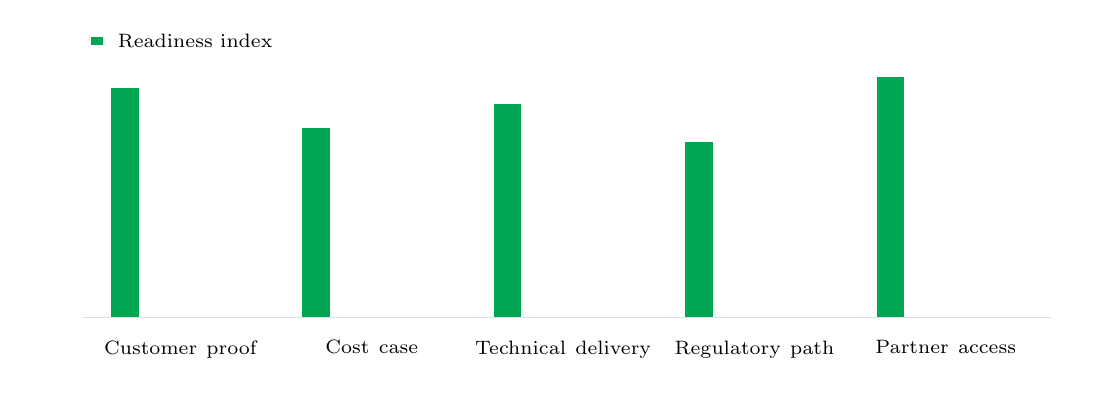
\begin{tikzpicture}[x=1cm,y=1cm]
\path[use as bounding box] (0,0) rectangle (13.20,4.40);
\draw[BOLine] (0.70,0.72) -- (13.00,0.72);
\fill[BOGreen] (1.06,0.72) rectangle (1.41,3.64);
\node[anchor=north,align=center,text width=2.24cm] at (1.94,0.55) {\scriptsize Customer proof};
\fill[BOGreen] (3.49,0.72) rectangle (3.84,3.13);
\node[anchor=north,align=center,text width=2.24cm] at (4.37,0.55) {\scriptsize Cost case};
\fill[BOGreen] (5.92,0.72) rectangle (6.27,3.43);
\node[anchor=north,align=center,text width=2.24cm] at (6.80,0.55) {\scriptsize Technical delivery};
\fill[BOGreen] (8.35,0.72) rectangle (8.70,2.95);
\node[anchor=north,align=center,text width=2.24cm] at (9.23,0.55) {\scriptsize Regulatory path};
\fill[BOGreen] (10.78,0.72) rectangle (11.13,3.77);
\node[anchor=north,align=center,text width=2.24cm] at (11.66,0.55) {\scriptsize Partner access};
\fill[BOGreen] (0.80,4.18) rectangle (0.96,4.28);
\node[anchor=west] at (1.02,4.23) {\scriptsize Readiness index};
\end{tikzpicture}\par\vspace{2pt}
\vspace{1pt}\noindent\begin{minipage}[t]{0.92\linewidth}
{\footnotesize\color{BOText} The exhibit ranks the proof points a CEO should ask teams to close before moving from monitoring to commitment.}\par
\end{minipage}\par\vspace{1pt}
\vspace{4pt}{\footnotesize\color{BOText} The exhibit ranks the proof points a CEO should ask teams to close before moving from monitoring to commitment.}\par
{\scriptsize\color{BOMuted} BlueOcean public-source synthesis.}\par
\vspace{9pt}\textcolor{BOLine}{\rule{\linewidth}{0.3pt}}\vspace{8pt}
{\textcolor{BOGreen}{\scriptsize\bfseries EXHIBIT 2}}\par\vspace{4pt}
{\sffamily\fontsize{17}{21}\selectfont\color{BONavy} Commitment posture should shift as proof matures}\par
{\small\color{BOText} Resource posture for Nuclear Fusion Commercialization: Strategic Implications for Energy Markets and Investment}\par\vspace{6pt}
\noindent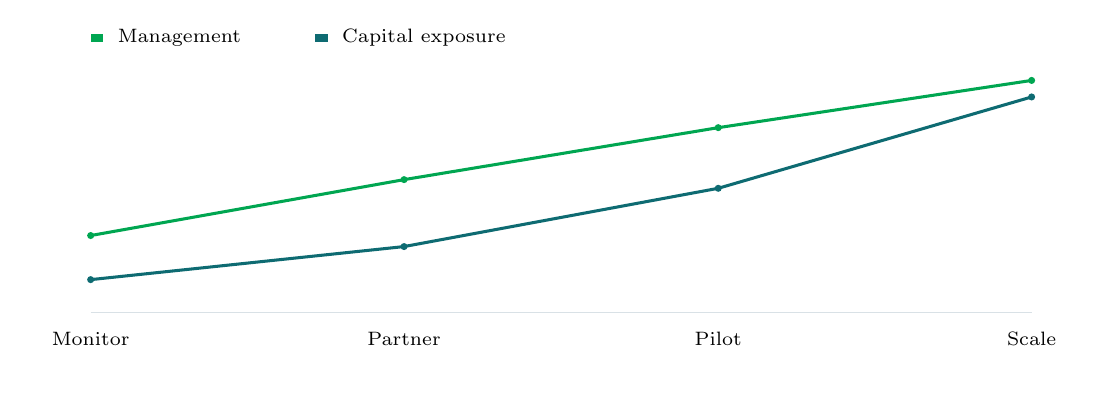
\begin{tikzpicture}[x=1cm,y=1cm]
\path[use as bounding box] (0,0) rectangle (13.20,4.40);
\draw[BOLine] (0.80,0.78) -- (12.75,0.78);
\draw[BOGreen,line width=1.1pt] (0.80,1.76) -- (4.78,2.47) -- (8.77,3.13) -- (12.75,3.73);
\fill[BOGreen] (0.80,1.76) circle (.045);
\fill[BOGreen] (4.78,2.47) circle (.045);
\fill[BOGreen] (8.77,3.13) circle (.045);
\fill[BOGreen] (12.75,3.73) circle (.045);
\draw[BOBlue,line width=1.1pt] (0.80,1.20) -- (4.78,1.62) -- (8.77,2.36) -- (12.75,3.52);
\fill[BOBlue] (0.80,1.20) circle (.045);
\fill[BOBlue] (4.78,1.62) circle (.045);
\fill[BOBlue] (8.77,2.36) circle (.045);
\fill[BOBlue] (12.75,3.52) circle (.045);
\node[anchor=north,align=center,text width=1.8cm] at (0.80,0.66) {\scriptsize Monitor};
\node[anchor=north,align=center,text width=1.8cm] at (4.78,0.66) {\scriptsize Partner};
\node[anchor=north,align=center,text width=1.8cm] at (8.77,0.66) {\scriptsize Pilot};
\node[anchor=north,align=center,text width=1.8cm] at (12.75,0.66) {\scriptsize Scale};
\fill[BOGreen] (0.80,4.22) rectangle (0.96,4.32);
\node[anchor=west] at (1.02,4.27) {\scriptsize Management};
\fill[BOBlue] (3.65,4.22) rectangle (3.81,4.32);
\node[anchor=west] at (3.87,4.27) {\scriptsize Capital exposure};
\end{tikzpicture}\par\vspace{2pt}
\vspace{1pt}\noindent\begin{minipage}[t]{0.92\linewidth}
{\footnotesize\color{BOText} Capital exposure should lag evidence maturity rather than lead it.}\par
\end{minipage}\par\vspace{1pt}
\vspace{4pt}{\footnotesize\color{BOText} Capital exposure should lag evidence maturity rather than lead it.}\par
{\scriptsize\color{BOMuted} BlueOcean scenario synthesis.}\par

\clearpage
\label{chap:2}
\noindent\begin{tikzpicture}
\path[use as bounding box] (0,0) rectangle (\linewidth,54mm);
\clip (0,0) rectangle (\linewidth,54mm);
\node[anchor=north west,inner sep=0] at (0,54mm) {
\includegraphics[width=\linewidth]{assets/image-2.png}};
\end{tikzpicture}
\vspace{0pt}
\noindent
\begin{tikzpicture}
\fill[BOGreen] (0,0) rectangle (96mm,1.2pt);
\end{tikzpicture}\par\vspace{8pt}
{\Large\sffamily\bfseries\color{BONavy} Economic Competitiveness Will Depend on Achieving Cost Targets Below \$50/MWh and High Availability}\par\vspace{4pt}
{\sffamily\fontsize{15}{20}\selectfont\color{BOGreen} For Economic Competitiveness Will Depend on Achieving Cost Targets Below \$50/MWh and High Availability, the next useful work is to convert the supporting sources into a short list of claims that would change capital timing,.}\par\vspace{9pt}
\begin{multicols}{2}
{\small For Economic Competitiveness Will Depend on Achieving Cost Targets Below \$50/MWh and High Availability, the next useful work is to convert the supporting sources into a short list of claims that would change capital timing, customer exposure or partner posture. Claims that do not change those decisions should stay out of the main narrative.}\par
{\small Commercial readiness should be judged through customer adoption, cost structure, delivery cycle, service capability and financing availability. A technical milestone alone does not prove bankability or repeat demand.}\par
{\small Management should require every major assumption to tie back to a verifiable claim: target customer, buying trigger, budget owner, substitute, use case and payback path. Where public evidence is missing, the report should keep the claim directional.}\par
{\small A more robust path is to build credible proof through pilots, partner diligence and third-party validation before moving into larger commitments.}\par
{\small The commercial implication is that the next review should test the chapter against customer evidence, cost data, policy timing and competitor movement, then update the investment threshold.}\par
\end{multicols}
\label{chap:2:end}

\clearpage
{\textcolor{BOGreen}{\scriptsize\bfseries EXHIBIT 3}}\par\vspace{4pt}
{\sffamily\fontsize{17}{21}\selectfont\color{BONavy} Key risks should be ranked by severity and manageability}\par
{\small\color{BOText} Risk exposure for Nuclear Fusion Commercialization: Strategic Implications for Energy Markets and Investment}\par\vspace{6pt}
\noindent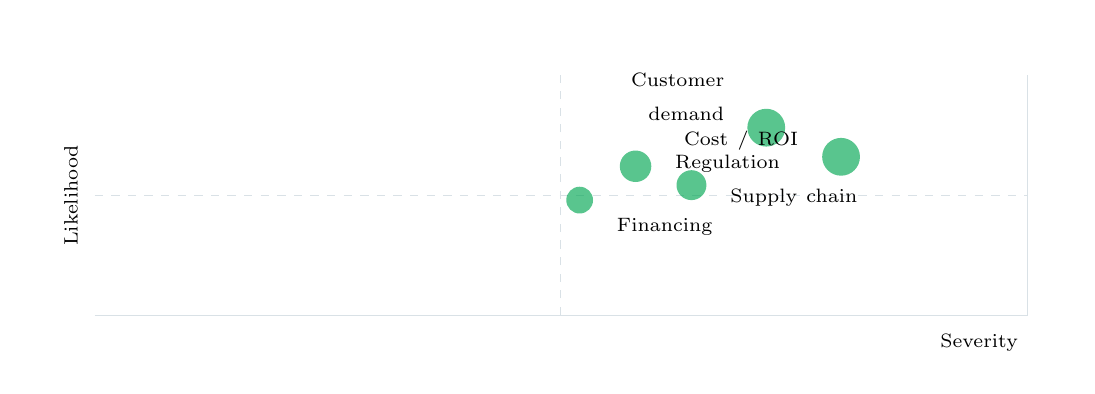
\begin{tikzpicture}[x=1cm,y=1cm]
\path[use as bounding box] (0,0) rectangle (13.20,4.30);
\draw[BOLine] (0.85,0.65) -- (12.70,0.65) -- (12.70,3.70);
\draw[BOLine,dashed] (0.85,2.17) -- (12.70,2.17);
\draw[BOLine,dashed] (6.77,0.65) -- (6.77,3.70);
\fill[BOGreen,opacity=.65] (9.38,3.03) circle (0.24);
\node[anchor=east,align=right,text width=2.10cm] at (8.97,3.42) {\scriptsize Customer demand};
\fill[BOGreen,opacity=.65] (10.33,2.66) circle (0.24);
\node[anchor=east,align=right,text width=2.10cm] at (9.91,2.87) {\scriptsize Cost / ROI};
\fill[BOGreen,opacity=.65] (7.72,2.54) circle (0.20);
\node[anchor=west,align=left,text width=2.10cm] at (8.10,2.57) {\scriptsize Regulation};
\fill[BOGreen,opacity=.65] (8.43,2.30) circle (0.19);
\node[anchor=west,align=left,text width=2.10cm] at (8.80,2.14) {\scriptsize Supply chain};
\fill[BOGreen,opacity=.65] (7.01,2.11) circle (0.17);
\node[anchor=west,align=left,text width=2.10cm] at (7.36,1.77) {\scriptsize Financing};
\node[anchor=north east] at (12.70,0.53) {\scriptsize Severity};
\node[anchor=center,rotate=90] at (0.55,2.17) {\scriptsize Likelihood};
\end{tikzpicture}\par\vspace{2pt}
\vspace{1pt}\noindent\begin{minipage}[t]{0.92\linewidth}
{\footnotesize\color{BOText} Bubble size indicates the management attention required.}\par
\end{minipage}\par\vspace{1pt}
\vspace{4pt}{\footnotesize\color{BOText} Bubble size indicates the management attention required.}\par
{\scriptsize\color{BOMuted} BlueOcean risk screen.}\par
\vspace{9pt}\textcolor{BOLine}{\rule{\linewidth}{0.3pt}}\vspace{8pt}
{\textcolor{BOGreen}{\scriptsize\bfseries EXHIBIT 4}}\par\vspace{4pt}
{\sffamily\fontsize{17}{21}\selectfont\color{BONavy} Diligence workload concentrates in customer, cost and policy proof}\par
{\small\color{BOText} Near-term validation load for Nuclear Fusion Commercialization: Strategic Implications for Energy Markets and Investment}\par\vspace{6pt}
\noindent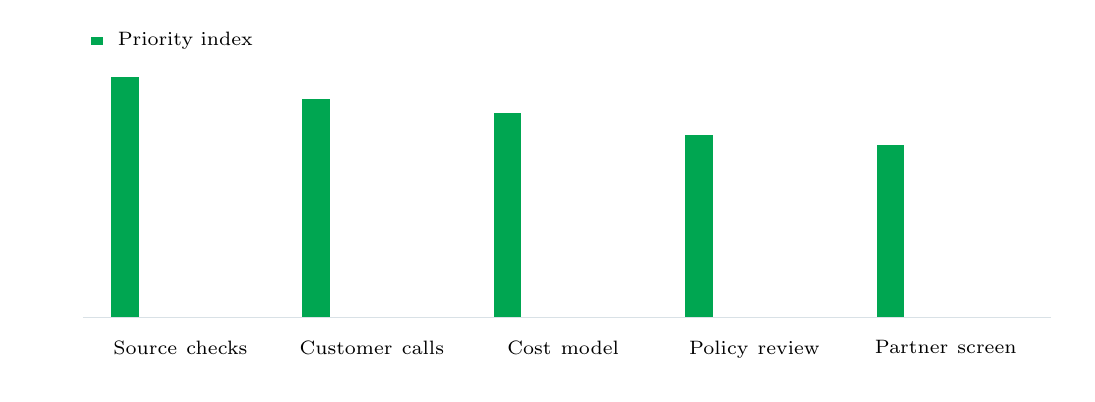
\begin{tikzpicture}[x=1cm,y=1cm]
\path[use as bounding box] (0,0) rectangle (13.20,4.40);
\draw[BOLine] (0.70,0.72) -- (13.00,0.72);
\fill[BOGreen] (1.06,0.72) rectangle (1.41,3.77);
\node[anchor=north,align=center,text width=2.24cm] at (1.94,0.55) {\scriptsize Source checks};
\fill[BOGreen] (3.49,0.72) rectangle (3.84,3.50);
\node[anchor=north,align=center,text width=2.24cm] at (4.37,0.55) {\scriptsize Customer calls};
\fill[BOGreen] (5.92,0.72) rectangle (6.27,3.31);
\node[anchor=north,align=center,text width=2.24cm] at (6.80,0.55) {\scriptsize Cost model};
\fill[BOGreen] (8.35,0.72) rectangle (8.70,3.04);
\node[anchor=north,align=center,text width=2.24cm] at (9.23,0.55) {\scriptsize Policy review};
\fill[BOGreen] (10.78,0.72) rectangle (11.13,2.91);
\node[anchor=north,align=center,text width=2.24cm] at (11.66,0.55) {\scriptsize Partner screen};
\fill[BOGreen] (0.80,4.18) rectangle (0.96,4.28);
\node[anchor=west] at (1.02,4.23) {\scriptsize Priority index};
\end{tikzpicture}\par\vspace{2pt}
\vspace{1pt}\noindent\begin{minipage}[t]{0.92\linewidth}
{\footnotesize\color{BOText} The most valuable work closes open questions that can change the decision.}\par
\end{minipage}\par\vspace{1pt}
\vspace{4pt}{\footnotesize\color{BOText} The most valuable work closes open questions that can change the decision.}\par
{\scriptsize\color{BOMuted} BlueOcean public-source synthesis.}\par

\clearpage
\label{chap:3}
\noindent\begin{tikzpicture}
\path[use as bounding box] (0,0) rectangle (\linewidth,54mm);
\clip (0,0) rectangle (\linewidth,54mm);
\node[anchor=north west,inner sep=0] at (0,54mm) {
\includegraphics[width=\linewidth]{assets/image-3.png}};
\end{tikzpicture}
\vspace{0pt}
\noindent
\begin{tikzpicture}
\fill[BOGreen] (0,0) rectangle (96mm,1.2pt);
\end{tikzpicture}\par\vspace{8pt}
{\Large\sffamily\bfseries\color{BONavy} Fusion Will Complement Renewables and Enable Hard-to-Decarbonize Sectors Like Heavy Industry}\par\vspace{4pt}
{\sffamily\fontsize{15}{20}\selectfont\color{BOGreen} For Fusion Will Complement Renewables and Enable Hard-to-Decarbonize Sectors Like Heavy Industry, the next useful work is to convert the supporting sources into a short list of claims that would change capital timing, custom.}\par\vspace{9pt}
\begin{multicols}{2}
{\small For Fusion Will Complement Renewables and Enable Hard-to-Decarbonize Sectors Like Heavy Industry, the next useful work is to convert the supporting sources into a short list of claims that would change capital timing, customer exposure or partner posture. Claims that do not change those decisions should stay out of the main narrative.}\par
{\small Every opportunity eventually returns to cost, revenue, margin, cash flow and timing. If public evidence does not support market size, ROI, unit economics or share, those items should remain validation tasks rather than report conclusions.}\par
{\small Near-term action should focus on verifiable cost drivers and customer willingness to pay instead of relying on optimistic long-range scenarios. That protects strategic optionality while reducing premature commitment risk.}\par
{\small As cost, customer and financing evidence improves, management can shift resources from monitoring and partnerships toward pilots or scaled deployment.}\par
{\small The board-level question is whether the next review should test the chapter against customer evidence, cost data, policy timing and competitor movement, then update the investment threshold.}\par
\end{multicols}
\label{chap:3:end}

\clearpage
{\textcolor{BOGreen}{\scriptsize\bfseries EXHIBIT 5}}\par\vspace{4pt}
{\sffamily\fontsize{17}{21}\selectfont\color{BONavy} Scenario choices should compare attractiveness with readiness}\par
{\small\color{BOText} Strategic option comparison for Nuclear Fusion Commercialization: Strategic Implications for Energy Markets and Investment}\par\vspace{6pt}
{\scriptsize\begin{tabular}{p{38mm}>{\centering\arraybackslash}p{21mm}>{\centering\arraybackslash}p{21mm}>{\centering\arraybackslash}p{21mm}>{\centering\arraybackslash}p{21mm}}
 & {\bfseries Attractiveness} & {\bfseries Readiness} & {\bfseries Confidence} & {\bfseries Capital need} \\
\hline
{\bfseries Fusion Commercialization Is} & \colorbox{BOGreen}{\textcolor{white}{\strut\hspace{5pt}5\hspace{5pt}}} & \colorbox{BOBlue}{\textcolor{white}{\strut\hspace{5pt}3\hspace{5pt}}} & \colorbox{BOLight}{\textcolor{BOText}{\strut\hspace{5pt}2\hspace{5pt}}} & \colorbox{BOLight}{\textcolor{BOText}{\strut\hspace{5pt}2\hspace{5pt}}} \\
{\bfseries Economic Competitiveness Will} & \colorbox{BOGreen}{\textcolor{white}{\strut\hspace{5pt}4\hspace{5pt}}} & \colorbox{BOGreen}{\textcolor{white}{\strut\hspace{5pt}4\hspace{5pt}}} & \colorbox{BOBlue}{\textcolor{white}{\strut\hspace{5pt}3\hspace{5pt}}} & \colorbox{BOBlue}{\textcolor{white}{\strut\hspace{5pt}3\hspace{5pt}}} \\
{\bfseries Fusion Will Complement} & \colorbox{BOGreen}{\textcolor{white}{\strut\hspace{5pt}4\hspace{5pt}}} & \colorbox{BOLight}{\textcolor{BOText}{\strut\hspace{5pt}2\hspace{5pt}}} & \colorbox{BOLight}{\textcolor{BOText}{\strut\hspace{5pt}2\hspace{5pt}}} & \colorbox{BOGreen}{\textcolor{white}{\strut\hspace{5pt}4\hspace{5pt}}} \\
{\bfseries Geopolitical Dynamics Will} & \colorbox{BOBlue}{\textcolor{white}{\strut\hspace{5pt}3\hspace{5pt}}} & \colorbox{BOBlue}{\textcolor{white}{\strut\hspace{5pt}3\hspace{5pt}}} & \colorbox{BOBlue}{\textcolor{white}{\strut\hspace{5pt}3\hspace{5pt}}} & \colorbox{BOLight}{\textcolor{BOText}{\strut\hspace{5pt}2\hspace{5pt}}} \\
{\bfseries Nuclear Fusion} & \colorbox{BOGreen}{\textcolor{white}{\strut\hspace{5pt}5\hspace{5pt}}} & \colorbox{BOBlue}{\textcolor{white}{\strut\hspace{5pt}3\hspace{5pt}}} & \colorbox{BOBlue}{\textcolor{white}{\strut\hspace{5pt}3\hspace{5pt}}} & \colorbox{BOBlue}{\textcolor{white}{\strut\hspace{5pt}3\hspace{5pt}}} \\
\end{tabular}}\par\vspace{2pt}
\vspace{1pt}\noindent\begin{minipage}[t]{0.92\linewidth}
{\footnotesize\color{BOText} The matrix ranks where the next validation work should focus.}\par
\end{minipage}\par\vspace{1pt}
\vspace{4pt}{\footnotesize\color{BOText} The matrix ranks where the next validation work should focus.}\par
{\scriptsize\color{BOMuted} BlueOcean qualitative assessment.}\par
\vspace{9pt}\textcolor{BOLine}{\rule{\linewidth}{0.3pt}}\vspace{8pt}
{\textcolor{BOGreen}{\scriptsize\bfseries EXHIBIT 6}}\par\vspace{4pt}
{\sffamily\fontsize{17}{21}\selectfont\color{BONavy} Validation effort shifts from customer proof to policy and partners}\par
{\small\color{BOText} Quarterly validation mix for Nuclear Fusion Commercialization: Strategic Implications for Energy Markets and Investment}\par\vspace{6pt}
\noindent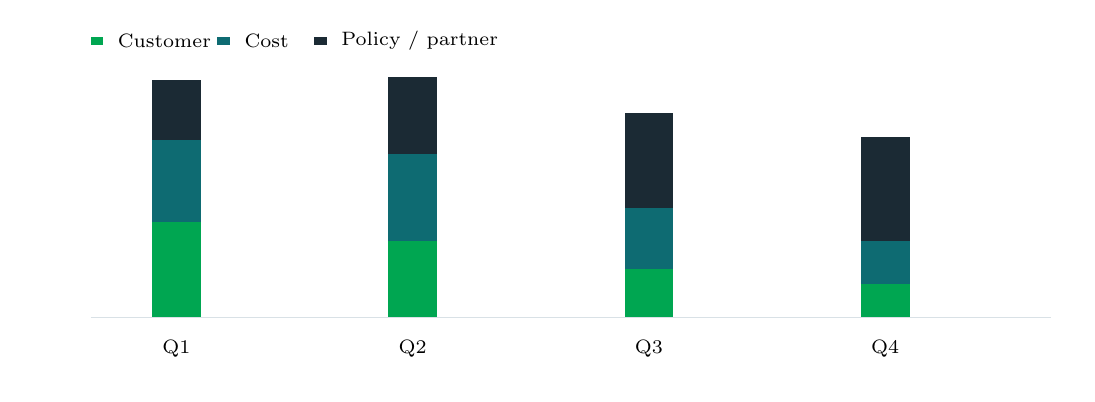
\begin{tikzpicture}[x=1cm,y=1cm]
\path[use as bounding box] (0,0) rectangle (13.20,4.40);
\draw[BOLine] (0.80,0.72) -- (13.00,0.72);
\fill[BOGreen] (1.58,0.72) rectangle (2.20,1.93);
\fill[BOBlue] (1.58,1.93) rectangle (2.20,2.97);
\fill[BONavy] (1.58,2.97) rectangle (2.20,3.74);
\node[anchor=north,align=center,text width=2.76cm] at (1.89,0.55) {\scriptsize Q1};
\fill[BOGreen] (4.58,0.72) rectangle (5.20,1.69);
\fill[BOBlue] (4.58,1.69) rectangle (5.20,2.80);
\fill[BONavy] (4.58,2.80) rectangle (5.20,3.77);
\node[anchor=north,align=center,text width=2.76cm] at (4.89,0.55) {\scriptsize Q2};
\fill[BOGreen] (7.58,0.72) rectangle (8.20,1.34);
\fill[BOBlue] (7.58,1.34) rectangle (8.20,2.11);
\fill[BONavy] (7.58,2.11) rectangle (8.20,3.32);
\node[anchor=north,align=center,text width=2.76cm] at (7.89,0.55) {\scriptsize Q3};
\fill[BOGreen] (10.58,0.72) rectangle (11.20,1.14);
\fill[BOBlue] (10.58,1.14) rectangle (11.20,1.69);
\fill[BONavy] (10.58,1.69) rectangle (11.20,3.01);
\node[anchor=north,align=center,text width=2.76cm] at (10.89,0.55) {\scriptsize Q4};
\fill[BOGreen] (0.80,4.18) rectangle (0.96,4.28);
\node[anchor=west] at (1.02,4.23) {\scriptsize Customer};
\fill[BOBlue] (2.41,4.18) rectangle (2.57,4.28);
\node[anchor=west] at (2.63,4.23) {\scriptsize Cost};
\fill[BONavy] (3.64,4.18) rectangle (3.80,4.28);
\node[anchor=west] at (3.86,4.23) {\scriptsize Policy / partner};
\end{tikzpicture}\par\vspace{2pt}
\vspace{1pt}\noindent\begin{minipage}[t]{0.92\linewidth}
{\footnotesize\color{BOText} The validation cadence should improve facts before escalating resource commitment.}\par
\end{minipage}\par\vspace{1pt}
\vspace{4pt}{\footnotesize\color{BOText} The validation cadence should improve facts before escalating resource commitment.}\par
{\scriptsize\color{BOMuted} BlueOcean public-source synthesis.}\par

\clearpage
\label{chap:4}
\noindent\begin{tikzpicture}
\path[use as bounding box] (0,0) rectangle (\linewidth,54mm);
\clip (0,0) rectangle (\linewidth,54mm);
\node[anchor=north west,inner sep=0] at (0,54mm) {
\includegraphics[width=\linewidth]{assets/image-4.png}};
\end{tikzpicture}
\vspace{0pt}
\noindent
\begin{tikzpicture}
\fill[BOGreen] (0,0) rectangle (96mm,1.2pt);
\end{tikzpicture}\par\vspace{8pt}
{\Large\sffamily\bfseries\color{BONavy} Geopolitical Dynamics Will Shift as Fusion Reduces Dependence on Fossil Fuel Exporters}\par\vspace{4pt}
{\sffamily\fontsize{15}{20}\selectfont\color{BOGreen} For Geopolitical Dynamics Will Shift as Fusion Reduces Dependence on Fossil Fuel Exporters, the next useful work is to convert the supporting sources into a short list of claims that would change capital timing, customer exp.}\par\vspace{9pt}
\begin{multicols}{2}
{\small For Geopolitical Dynamics Will Shift as Fusion Reduces Dependence on Fossil Fuel Exporters, the next useful work is to convert the supporting sources into a short list of claims that would change capital timing, customer exposure or partner posture. Claims that do not change those decisions should stay out of the main narrative.}\par
{\small Policy support, permitting rules, standards and public acceptance affect how quickly an opportunity moves from concept to deployment. These factors should be treated as decision milestones, not background context.}\par
{\small Where the regulatory path is unclear, the better move is usually standards engagement, policy tracking and low-risk pilots rather than an early heavy-asset commitment.}\par
{\small The board should track which policy events would change investment timing, such as licensing rules, procurement requirements, subsidy treatment, local approvals or safety standards.}\par
{\small For leadership teams, the next review should test the chapter against customer evidence, cost data, policy timing and competitor movement, then update the investment threshold.}\par
\end{multicols}
\label{chap:4:end}

\clearpage
{\textcolor{BOGreen}{\scriptsize\bfseries EXHIBIT 7}}\par\vspace{4pt}
{\sffamily\fontsize{17}{21}\selectfont\color{BONavy} Cost structure must be decomposed before underwriting}\par
{\small\color{BOText} Cost diligence view for Nuclear Fusion Commercialization: Strategic Implications for Energy Markets and Investment}\par\vspace{6pt}
\noindent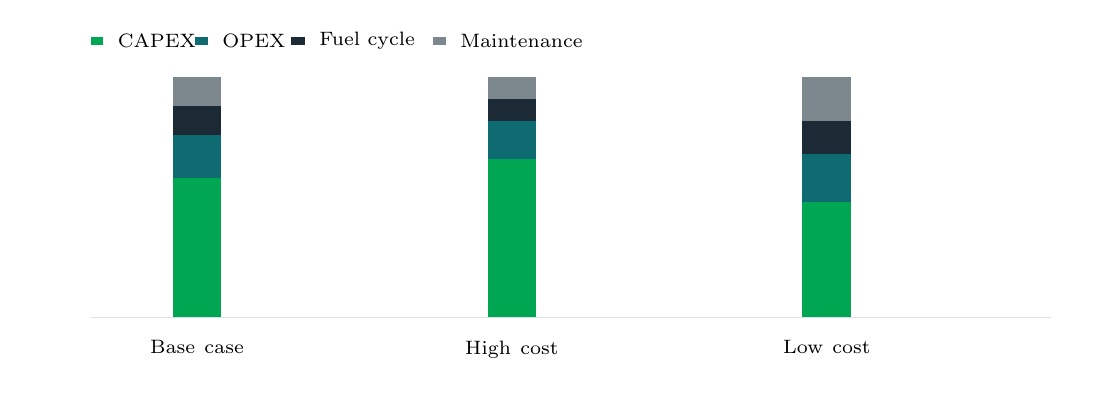
\begin{tikzpicture}[x=1cm,y=1cm]
\path[use as bounding box] (0,0) rectangle (13.20,4.40);
\draw[BOLine] (0.80,0.72) -- (13.00,0.72);
\fill[BOGreen] (1.84,0.72) rectangle (2.46,2.49);
\fill[BOBlue] (1.84,2.49) rectangle (2.46,3.04);
\fill[BONavy] (1.84,3.04) rectangle (2.46,3.40);
\fill[BOMuted] (1.84,3.40) rectangle (2.46,3.77);
\node[anchor=north,align=center,text width=3.68cm] at (2.15,0.55) {\scriptsize Base case};
\fill[BOGreen] (5.84,0.72) rectangle (6.46,2.73);
\fill[BOBlue] (5.84,2.73) rectangle (6.46,3.22);
\fill[BONavy] (5.84,3.22) rectangle (6.46,3.50);
\fill[BOMuted] (5.84,3.50) rectangle (6.46,3.77);
\node[anchor=north,align=center,text width=3.68cm] at (6.15,0.55) {\scriptsize High cost};
\fill[BOGreen] (9.84,0.72) rectangle (10.46,2.18);
\fill[BOBlue] (9.84,2.18) rectangle (10.46,2.79);
\fill[BONavy] (9.84,2.79) rectangle (10.46,3.22);
\fill[BOMuted] (9.84,3.22) rectangle (10.46,3.77);
\node[anchor=north,align=center,text width=3.68cm] at (10.15,0.55) {\scriptsize Low cost};
\fill[BOGreen] (0.80,4.18) rectangle (0.96,4.28);
\node[anchor=west] at (1.02,4.23) {\scriptsize CAPEX};
\fill[BOBlue] (2.12,4.18) rectangle (2.29,4.28);
\node[anchor=west] at (2.35,4.23) {\scriptsize OPEX};
\fill[BONavy] (3.35,4.18) rectangle (3.52,4.28);
\node[anchor=west] at (3.58,4.23) {\scriptsize Fuel cycle};
\fill[BOMuted] (5.15,4.18) rectangle (5.31,4.28);
\node[anchor=west] at (5.37,4.23) {\scriptsize Maintenance};
\end{tikzpicture}\par\vspace{2pt}
\vspace{1pt}\noindent\begin{minipage}[t]{0.92\linewidth}
{\footnotesize\color{BOText} The chart separates capital, operating and maintenance drivers so management can test which cost lever would change the investment case.}\par
\end{minipage}\par\vspace{1pt}
\vspace{4pt}{\footnotesize\color{BOText} The chart separates capital, operating and maintenance drivers so management can test which cost lever would change the investment case.}\par
{\scriptsize\color{BOMuted} BlueOcean public-source synthesis.}\par
\vspace{9pt}\textcolor{BOLine}{\rule{\linewidth}{0.3pt}}\vspace{8pt}
{\textcolor{BOGreen}{\scriptsize\bfseries EXHIBIT 8}}\par\vspace{4pt}
{\sffamily\fontsize{17}{21}\selectfont\color{BONavy} Timeline confidence falls as milestones move from lab to grid}\par
{\small\color{BOText} Milestone confidence for Nuclear Fusion Commercialization: Strategic Implications for Energy Markets and Investment}\par\vspace{6pt}
\noindent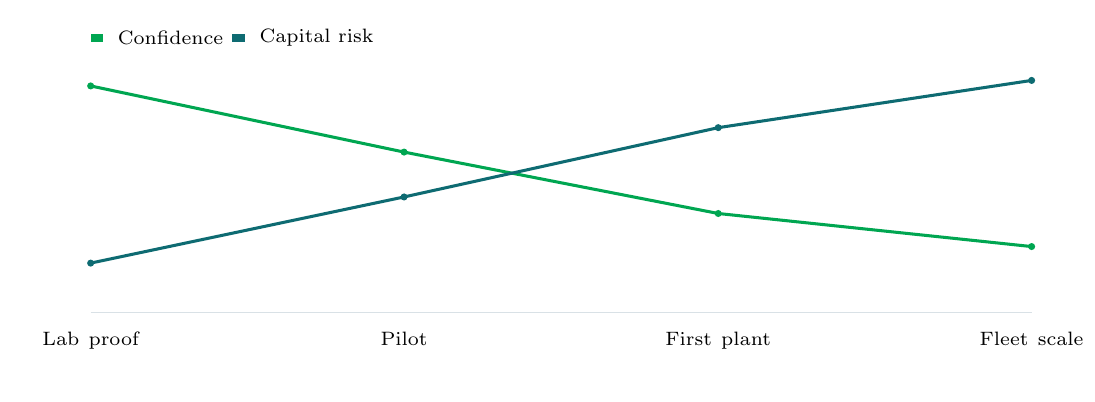
\begin{tikzpicture}[x=1cm,y=1cm]
\path[use as bounding box] (0,0) rectangle (13.20,4.40);
\draw[BOLine] (0.80,0.78) -- (12.75,0.78);
\draw[BOGreen,line width=1.1pt] (0.80,3.66) -- (4.78,2.82) -- (8.77,2.04) -- (12.75,1.62);
\fill[BOGreen] (0.80,3.66) circle (.045);
\fill[BOGreen] (4.78,2.82) circle (.045);
\fill[BOGreen] (8.77,2.04) circle (.045);
\fill[BOGreen] (12.75,1.62) circle (.045);
\draw[BOBlue,line width=1.1pt] (0.80,1.41) -- (4.78,2.25) -- (8.77,3.13) -- (12.75,3.73);
\fill[BOBlue] (0.80,1.41) circle (.045);
\fill[BOBlue] (4.78,2.25) circle (.045);
\fill[BOBlue] (8.77,3.13) circle (.045);
\fill[BOBlue] (12.75,3.73) circle (.045);
\node[anchor=north,align=center,text width=1.8cm] at (0.80,0.66) {\scriptsize Lab proof};
\node[anchor=north,align=center,text width=1.8cm] at (4.78,0.66) {\scriptsize Pilot};
\node[anchor=north,align=center,text width=1.8cm] at (8.77,0.66) {\scriptsize First plant};
\node[anchor=north,align=center,text width=1.8cm] at (12.75,0.66) {\scriptsize Fleet scale};
\fill[BOGreen] (0.80,4.22) rectangle (0.96,4.32);
\node[anchor=west] at (1.02,4.27) {\scriptsize Confidence};
\fill[BOBlue] (2.60,4.22) rectangle (2.76,4.32);
\node[anchor=west] at (2.82,4.27) {\scriptsize Capital risk};
\end{tikzpicture}\par\vspace{2pt}
\vspace{1pt}\noindent\begin{minipage}[t]{0.92\linewidth}
{\footnotesize\color{BOText} Decision confidence should be staged by milestone maturity.}\par
\end{minipage}\par\vspace{1pt}
\vspace{4pt}{\footnotesize\color{BOText} Decision confidence should be staged by milestone maturity.}\par
{\scriptsize\color{BOMuted} BlueOcean milestone assessment.}\par

\clearpage
\label{chap:5}
\noindent\begin{tikzpicture}
\path[use as bounding box] (0,0) rectangle (\linewidth,54mm);
\clip (0,0) rectangle (\linewidth,54mm);
\node[anchor=north west,inner sep=0] at (0,54mm) {
\includegraphics[width=\linewidth]{assets/image-5.png}};
\end{tikzpicture}
\vspace{0pt}
\noindent
\begin{tikzpicture}
\fill[BOGreen] (0,0) rectangle (96mm,1.2pt);
\end{tikzpicture}\par\vspace{8pt}
{\Large\sffamily\bfseries\color{BONavy} Nuclear Fusion Commercialization: Strategic Implications for Energy Markets and Investment should be managed as a staged strategic option, not a binary bet}\par\vspace{4pt}
{\sffamily\fontsize{15}{20}\selectfont\color{BOGreen} The CEO question is which moves are safe now and which should wait for stronger evidence.}\par\vspace{9pt}
\begin{multicols}{2}
{\small From a board perspective, for leadership, Nuclear Fusion Commercialization: Strategic Implications for Energy Markets and Investment should be separated into verified facts, directional scenarios and open diligence items. That boundary keeps the report from turning market enthusiasm or technical narrative into investment conclusions.}\par
{\small The commercial implication is that the immediate management question is not whether the opportunity is exciting; it is whether budget, partner access or management attention should be committed now. Low-cost validation can start early, while larger capital commitments should wait for customer, cost, financing, regulatory or operating proof.}\par
{\small The board-level question is whether the current evidence posture is: Public evidence retained in the supporting sources; additional validation is required for unsupported claims. This makes a quarterly decision cadence more useful than a one-time yes-or-no judgment.}\par
{\small For a CEO, Nuclear Fusion Commercialization: Strategic Implications for Energy Markets and Investment should be managed as a stage. matters only if it changes the timing of capital, partner access, customer commitments or risk appetite. The strongest posture is to keep learning close to the business while reserving heavier commitments for proof that can survive investment-committee scrutiny.}\par
{\small For Nuclear Fusion Commercialization: Strategic Implications for Energy Markets and Investment should be managed as a stage., resource allocation should follow the facts that can change the decision: customer demand, cost position, financing availability, regulatory path and delivery capability. If those facts do not improve, increasing exposure mainly creates strategic lock-in rather than higher conviction.}\par
\end{multicols}
\label{chap:5:end}

\clearpage
{\textcolor{BOGreen}{\scriptsize\bfseries EXHIBIT 9}}\par\vspace{4pt}
{\sffamily\fontsize{17}{21}\selectfont\color{BONavy} Partner options differ on learning value and capital exposure}\par
{\small\color{BOText} Where-to-play option view for Nuclear Fusion Commercialization: Strategic Implications for Energy Markets and Investment}\par\vspace{6pt}
{\scriptsize\begin{tabular}{p{38mm}>{\centering\arraybackslash}p{21mm}>{\centering\arraybackslash}p{21mm}>{\centering\arraybackslash}p{21mm}>{\centering\arraybackslash}p{21mm}}
 & {\bfseries Learning} & {\bfseries Control} & {\bfseries Capital need} & {\bfseries Reversibility} \\
\hline
{\bfseries Direct equity} & \colorbox{BOGreen}{\textcolor{white}{\strut\hspace{5pt}5\hspace{5pt}}} & \colorbox{BOGreen}{\textcolor{white}{\strut\hspace{5pt}4\hspace{5pt}}} & \colorbox{BOLight}{\textcolor{BOText}{\strut\hspace{5pt}2\hspace{5pt}}} & \colorbox{BOLight}{\textcolor{BOText}{\strut\hspace{5pt}2\hspace{5pt}}} \\
{\bfseries Corporate venture} & \colorbox{BOGreen}{\textcolor{white}{\strut\hspace{5pt}4\hspace{5pt}}} & \colorbox{BOBlue}{\textcolor{white}{\strut\hspace{5pt}3\hspace{5pt}}} & \colorbox{BOBlue}{\textcolor{white}{\strut\hspace{5pt}3\hspace{5pt}}} & \colorbox{BOBlue}{\textcolor{white}{\strut\hspace{5pt}3\hspace{5pt}}} \\
{\bfseries Offtake option} & \colorbox{BOBlue}{\textcolor{white}{\strut\hspace{5pt}3\hspace{5pt}}} & \colorbox{BOLight}{\textcolor{BOText}{\strut\hspace{5pt}2\hspace{5pt}}} & \colorbox{BOGreen}{\textcolor{white}{\strut\hspace{5pt}4\hspace{5pt}}} & \colorbox{BOGreen}{\textcolor{white}{\strut\hspace{5pt}4\hspace{5pt}}} \\
{\bfseries Supplier JV} & \colorbox{BOGreen}{\textcolor{white}{\strut\hspace{5pt}4\hspace{5pt}}} & \colorbox{BOGreen}{\textcolor{white}{\strut\hspace{5pt}4\hspace{5pt}}} & \colorbox{BOLight}{\textcolor{BOText}{\strut\hspace{5pt}2\hspace{5pt}}} & \colorbox{BOLight}{\textcolor{BOText}{\strut\hspace{5pt}2\hspace{5pt}}} \\
{\bfseries R\&D consortium} & \colorbox{BOBlue}{\textcolor{white}{\strut\hspace{5pt}3\hspace{5pt}}} & \colorbox{BOLight}{\textcolor{BOText}{\strut\hspace{5pt}2\hspace{5pt}}} & \colorbox{BOGreen}{\textcolor{white}{\strut\hspace{5pt}5\hspace{5pt}}} & \colorbox{BOGreen}{\textcolor{white}{\strut\hspace{5pt}5\hspace{5pt}}} \\
\end{tabular}}\par\vspace{2pt}
\vspace{1pt}\noindent\begin{minipage}[t]{0.92\linewidth}
{\footnotesize\color{BOText} The best early posture maximizes learning without forcing irreversible capital exposure.}\par
\end{minipage}\par\vspace{1pt}
\vspace{4pt}{\footnotesize\color{BOText} The best early posture maximizes learning without forcing irreversible capital exposure.}\par
{\scriptsize\color{BOMuted} BlueOcean option synthesis.}\par
\vspace{9pt}\textcolor{BOLine}{\rule{\linewidth}{0.3pt}}\vspace{8pt}
{\textcolor{BOGreen}{\scriptsize\bfseries EXHIBIT 10}}\par\vspace{4pt}
{\sffamily\fontsize{17}{21}\selectfont\color{BONavy} Evidence maturity varies sharply by claim type}\par
{\small\color{BOText} Claim maturity for Nuclear Fusion Commercialization: Strategic Implications for Energy Markets and Investment}\par\vspace{6pt}
\noindent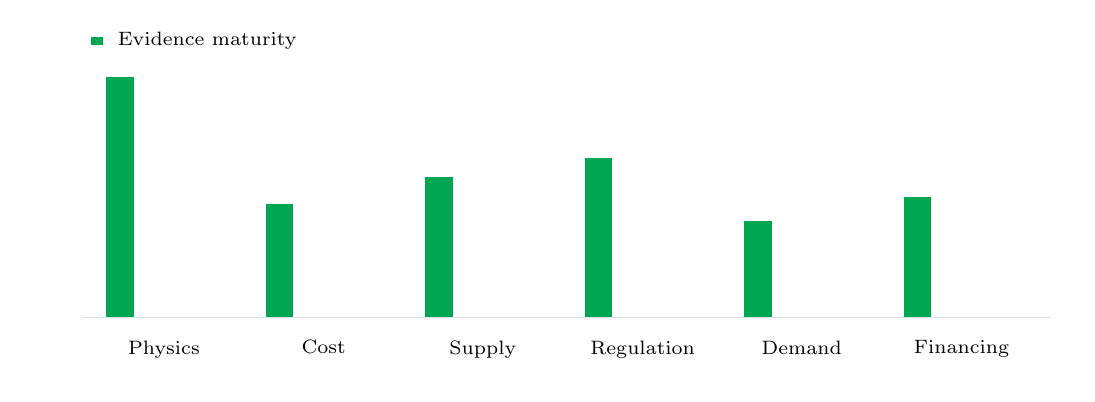
\begin{tikzpicture}[x=1cm,y=1cm]
\path[use as bounding box] (0,0) rectangle (13.20,4.40);
\draw[BOLine] (0.70,0.72) -- (13.00,0.72);
\fill[BOGreen] (1.00,0.72) rectangle (1.35,3.77);
\node[anchor=north,align=center,text width=1.86cm] at (1.73,0.55) {\scriptsize Physics};
\fill[BOGreen] (3.03,0.72) rectangle (3.37,2.16);
\node[anchor=north,align=center,text width=1.86cm] at (3.76,0.55) {\scriptsize Cost};
\fill[BOGreen] (5.05,0.72) rectangle (5.40,2.50);
\node[anchor=north,align=center,text width=1.86cm] at (5.78,0.55) {\scriptsize Supply};
\fill[BOGreen] (7.08,0.72) rectangle (7.42,2.75);
\node[anchor=north,align=center,text width=1.86cm] at (7.81,0.55) {\scriptsize Regulation};
\fill[BOGreen] (9.10,0.72) rectangle (9.45,1.95);
\node[anchor=north,align=center,text width=1.86cm] at (9.83,0.55) {\scriptsize Demand};
\fill[BOGreen] (11.13,0.72) rectangle (11.47,2.25);
\node[anchor=north,align=center,text width=1.86cm] at (11.86,0.55) {\scriptsize Financing};
\fill[BOGreen] (0.80,4.18) rectangle (0.96,4.28);
\node[anchor=west] at (1.02,4.23) {\scriptsize Evidence maturity};
\end{tikzpicture}\par\vspace{2pt}
\vspace{1pt}\noindent\begin{minipage}[t]{0.92\linewidth}
{\footnotesize\color{BOText} Management can use the maturity gap to decide which claims support action today and which require a separate diligence workstream.}\par
\end{minipage}\par\vspace{1pt}
\vspace{4pt}{\footnotesize\color{BOText} Management can use the maturity gap to decide which claims support action today and which require a separate diligence workstream.}\par
{\scriptsize\color{BOMuted} BlueOcean public-source synthesis.}\par

\clearpage
\label{chap:6}
\noindent\begin{tikzpicture}
\path[use as bounding box] (0,0) rectangle (\linewidth,54mm);
\clip (0,0) rectangle (\linewidth,54mm);
\node[anchor=north west,inner sep=0] at (0,54mm) {
\includegraphics[width=\linewidth]{assets/image-6.png}};
\end{tikzpicture}
\vspace{0pt}
\noindent
\begin{tikzpicture}
\fill[BOGreen] (0,0) rectangle (96mm,1.2pt);
\end{tikzpicture}\par\vspace{8pt}
{\Large\sffamily\bfseries\color{BONavy} Commercial readiness depends on bankability, deliverability and repeat customer proof}\par\vspace{4pt}
{\sffamily\fontsize{15}{20}\selectfont\color{BOGreen} Technical feasibility matters only when it changes customer value, cost position and execution confidence.}\par\vspace{9pt}
\begin{multicols}{2}
{\small The commercial implication is that commercial readiness should be judged through customer adoption, cost structure, delivery cycle, service capability and financing availability. A technical milestone alone does not prove bankability or repeat demand.}\par
{\small The board-level question is whether management should require every major assumption to tie back to a verifiable claim: target customer, buying trigger, budget owner, substitute, use case and payback path. Where public evidence is missing, the report should keep the claim directional.}\par
{\small For leadership teams, a more robust path is to build credible proof through pilots, partner diligence and third-party validation before moving into larger commitments.}\par
{\small For a CEO, Commercial readiness depends on bankability, deliverability and repeat customer proof matters only if it changes the timing of capital, partner access, customer commitments or risk appetite. The strongest posture is to keep learning close to the business while reserving heavier commitments for proof that can survive investment-committee scrutiny.}\par
{\small For Commercial readiness depends on bankability, deliverability and repeat customer proof, resource allocation should follow the facts that can change the decision: customer demand, cost position, financing availability, regulatory path and delivery capability. If those facts do not improve, increasing exposure mainly creates strategic lock-in rather than higher conviction.}\par
\end{multicols}
\label{chap:6:end}

\clearpage
{\textcolor{BOGreen}{\scriptsize\bfseries EXHIBIT 11}}\par\vspace{4pt}
{\sffamily\fontsize{17}{21}\selectfont\color{BONavy} Use-case priorities separate early revenue from long-term optionality}\par
{\small\color{BOText} Customer option screen for Nuclear Fusion Commercialization: Strategic Implications for Energy Markets and Investment}\par\vspace{6pt}
{\scriptsize\begin{tabular}{p{38mm}>{\centering\arraybackslash}p{21mm}>{\centering\arraybackslash}p{21mm}>{\centering\arraybackslash}p{21mm}>{\centering\arraybackslash}p{21mm}}
 & {\bfseries Demand pull} & {\bfseries Price tolerance} & {\bfseries Timing} & {\bfseries Evidence} \\
\hline
{\bfseries Industrial heat} & \colorbox{BOGreen}{\textcolor{white}{\strut\hspace{5pt}5\hspace{5pt}}} & \colorbox{BOGreen}{\textcolor{white}{\strut\hspace{5pt}4\hspace{5pt}}} & \colorbox{BOBlue}{\textcolor{white}{\strut\hspace{5pt}3\hspace{5pt}}} & \colorbox{BOBlue}{\textcolor{white}{\strut\hspace{5pt}3\hspace{5pt}}} \\
{\bfseries Hydrogen} & \colorbox{BOGreen}{\textcolor{white}{\strut\hspace{5pt}4\hspace{5pt}}} & \colorbox{BOGreen}{\textcolor{white}{\strut\hspace{5pt}4\hspace{5pt}}} & \colorbox{BOBlue}{\textcolor{white}{\strut\hspace{5pt}3\hspace{5pt}}} & \colorbox{BOLight}{\textcolor{BOText}{\strut\hspace{5pt}2\hspace{5pt}}} \\
{\bfseries Grid power} & \colorbox{BOGreen}{\textcolor{white}{\strut\hspace{5pt}5\hspace{5pt}}} & \colorbox{BOLight}{\textcolor{BOText}{\strut\hspace{5pt}2\hspace{5pt}}} & \colorbox{BOLight}{\textcolor{BOText}{\strut\hspace{5pt}1\hspace{5pt}}} & \colorbox{BOLight}{\textcolor{BOText}{\strut\hspace{5pt}2\hspace{5pt}}} \\
{\bfseries Defense / remote} & \colorbox{BOBlue}{\textcolor{white}{\strut\hspace{5pt}3\hspace{5pt}}} & \colorbox{BOGreen}{\textcolor{white}{\strut\hspace{5pt}5\hspace{5pt}}} & \colorbox{BOBlue}{\textcolor{white}{\strut\hspace{5pt}3\hspace{5pt}}} & \colorbox{BOLight}{\textcolor{BOText}{\strut\hspace{5pt}2\hspace{5pt}}} \\
{\bfseries Research services} & \colorbox{BOLight}{\textcolor{BOText}{\strut\hspace{5pt}2\hspace{5pt}}} & \colorbox{BOBlue}{\textcolor{white}{\strut\hspace{5pt}3\hspace{5pt}}} & \colorbox{BOGreen}{\textcolor{white}{\strut\hspace{5pt}4\hspace{5pt}}} & \colorbox{BOGreen}{\textcolor{white}{\strut\hspace{5pt}4\hspace{5pt}}} \\
\end{tabular}}\par\vspace{2pt}
\vspace{1pt}\noindent\begin{minipage}[t]{0.92\linewidth}
{\footnotesize\color{BOText} The comparison separates markets that can teach the company soon from markets that may require longer proof cycles.}\par
\end{minipage}\par\vspace{1pt}
\vspace{4pt}{\footnotesize\color{BOText} The comparison separates markets that can teach the company soon from markets that may require longer proof cycles.}\par
{\scriptsize\color{BOMuted} BlueOcean customer option synthesis.}\par
\vspace{9pt}\textcolor{BOLine}{\rule{\linewidth}{0.3pt}}\vspace{8pt}
{\textcolor{BOGreen}{\scriptsize\bfseries EXHIBIT 12}}\par\vspace{4pt}
{\sffamily\fontsize{17}{21}\selectfont\color{BONavy} Capital exposure should be staged by decision milestone}\par
{\small\color{BOText} Commitment profile for Nuclear Fusion Commercialization: Strategic Implications for Energy Markets and Investment}\par\vspace{6pt}
\noindent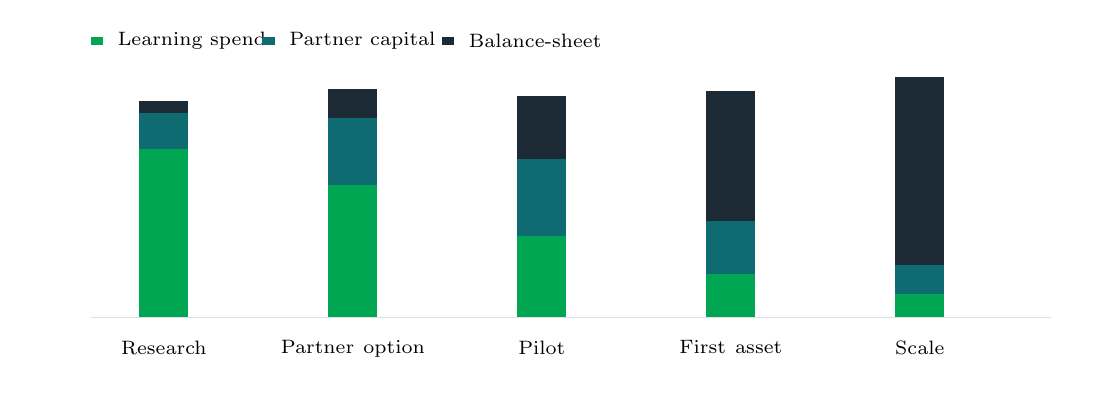
\begin{tikzpicture}[x=1cm,y=1cm]
\path[use as bounding box] (0,0) rectangle (13.20,4.40);
\draw[BOLine] (0.80,0.72) -- (13.00,0.72);
\fill[BOGreen] (1.42,0.72) rectangle (2.04,2.86);
\fill[BOBlue] (1.42,2.86) rectangle (2.04,3.31);
\fill[BONavy] (1.42,3.31) rectangle (2.04,3.47);
\node[anchor=north,align=center,text width=2.21cm] at (1.73,0.55) {\scriptsize Research};
\fill[BOGreen] (3.82,0.72) rectangle (4.44,2.40);
\fill[BOBlue] (3.82,2.40) rectangle (4.44,3.25);
\fill[BONavy] (3.82,3.25) rectangle (4.44,3.62);
\node[anchor=north,align=center,text width=2.21cm] at (4.13,0.55) {\scriptsize Partner option};
\fill[BOGreen] (6.22,0.72) rectangle (6.84,1.76);
\fill[BOBlue] (6.22,1.76) rectangle (6.84,2.73);
\fill[BONavy] (6.22,2.73) rectangle (6.84,3.53);
\node[anchor=north,align=center,text width=2.21cm] at (6.53,0.55) {\scriptsize Pilot};
\fill[BOGreen] (8.62,0.72) rectangle (9.24,1.27);
\fill[BOBlue] (8.62,1.27) rectangle (9.24,1.94);
\fill[BONavy] (8.62,1.94) rectangle (9.24,3.59);
\node[anchor=north,align=center,text width=2.21cm] at (8.93,0.55) {\scriptsize First asset};
\fill[BOGreen] (11.02,0.72) rectangle (11.64,1.02);
\fill[BOBlue] (11.02,1.02) rectangle (11.64,1.39);
\fill[BONavy] (11.02,1.39) rectangle (11.64,3.77);
\node[anchor=north,align=center,text width=2.21cm] at (11.33,0.55) {\scriptsize Scale};
\fill[BOGreen] (0.80,4.18) rectangle (0.96,4.28);
\node[anchor=west] at (1.02,4.23) {\scriptsize Learning spend};
\fill[BOBlue] (2.98,4.18) rectangle (3.14,4.28);
\node[anchor=west] at (3.20,4.23) {\scriptsize Partner capital};
\fill[BONavy] (5.26,4.18) rectangle (5.42,4.28);
\node[anchor=west] at (5.48,4.23) {\scriptsize Balance-sheet};
\end{tikzpicture}\par\vspace{2pt}
\vspace{1pt}\noindent\begin{minipage}[t]{0.92\linewidth}
{\footnotesize\color{BOText} The capital mix should move from learning to committed exposure only as evidence matures.}\par
\end{minipage}\par\vspace{1pt}
\vspace{4pt}{\footnotesize\color{BOText} The capital mix should move from learning to committed exposure only as evidence matures.}\par
{\scriptsize\color{BOMuted} BlueOcean capital staging view.}\par

\clearpage
\label{chap:7}
\noindent\begin{tikzpicture}
\path[use as bounding box] (0,0) rectangle (\linewidth,54mm);
\clip (0,0) rectangle (\linewidth,54mm);
\node[anchor=north west,inner sep=0] at (0,54mm) {
\includegraphics[width=\linewidth]{assets/image-7.png}};
\end{tikzpicture}
\vspace{0pt}
\noindent
\begin{tikzpicture}
\fill[BOGreen] (0,0) rectangle (96mm,1.2pt);
\end{tikzpicture}\par\vspace{8pt}
{\Large\sffamily\bfseries\color{BONavy} Cost, return and timing will determine the real deployment window}\par\vspace{4pt}
{\sffamily\fontsize{15}{20}\selectfont\color{BOGreen} Market size should not enter an investment case until the cost and return logic can be checked.}\par\vspace{9pt}
\begin{multicols}{2}
{\small The board-level question is whether every opportunity eventually returns to cost, revenue, margin, cash flow and timing. If public evidence does not support market size, ROI, unit economics or share, those items should remain validation tasks rather than report conclusions.}\par
{\small For leadership teams, near-term action should focus on verifiable cost drivers and customer willingness to pay instead of relying on optimistic long-range scenarios. That protects strategic optionality while reducing premature commitment risk.}\par
{\small A practical reading is that as cost, customer and financing evidence improves, management can shift resources from monitoring and partnerships toward pilots or scaled deployment.}\par
{\small For a CEO, Cost, return and timing will determine the real deployment window matters only if it changes the timing of capital, partner access, customer commitments or risk appetite. The strongest posture is to keep learning close to the business while reserving heavier commitments for proof that can survive investment-committee scrutiny.}\par
{\small For Cost, return and timing will determine the real deployment window, resource allocation should follow the facts that can change the decision: customer demand, cost position, financing availability, regulatory path and delivery capability. If those facts do not improve, increasing exposure mainly creates strategic lock-in rather than higher conviction.}\par
\end{multicols}
\label{chap:7:end}

\clearpage
{\textcolor{BOGreen}{\scriptsize\bfseries EXHIBIT 13}}\par\vspace{4pt}
{\sffamily\fontsize{17}{21}\selectfont\color{BONavy} Management attention shifts as the uncertainty stack resolves}\par
{\small\color{BOText} Executive review cadence for Nuclear Fusion Commercialization: Strategic Implications for Energy Markets and Investment}\par\vspace{6pt}
\noindent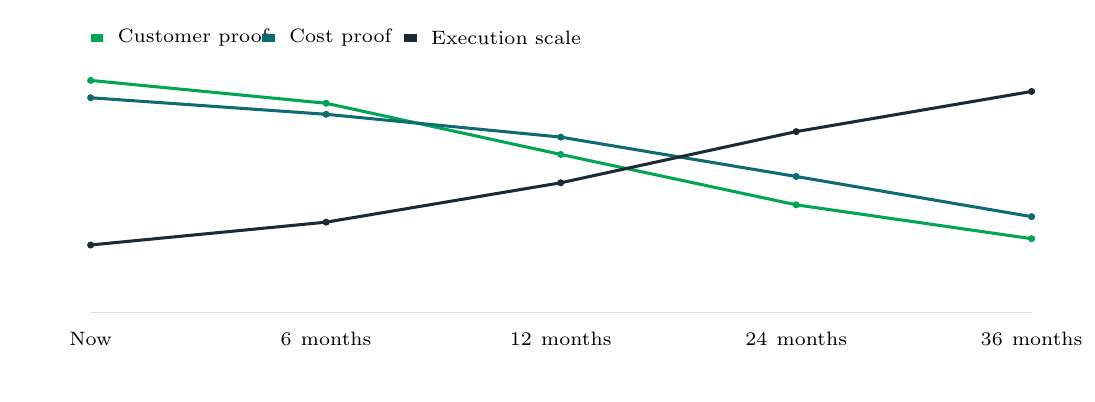
\begin{tikzpicture}[x=1cm,y=1cm]
\path[use as bounding box] (0,0) rectangle (13.20,4.40);
\draw[BOLine] (0.80,0.78) -- (12.75,0.78);
\draw[BOGreen,line width=1.1pt] (0.80,3.73) -- (3.79,3.44) -- (6.77,2.79) -- (9.76,2.15) -- (12.75,1.72);
\fill[BOGreen] (0.80,3.73) circle (.045);
\fill[BOGreen] (3.79,3.44) circle (.045);
\fill[BOGreen] (6.77,2.79) circle (.045);
\fill[BOGreen] (9.76,2.15) circle (.045);
\fill[BOGreen] (12.75,1.72) circle (.045);
\draw[BOBlue,line width=1.1pt] (0.80,3.51) -- (3.79,3.30) -- (6.77,3.01) -- (9.76,2.51) -- (12.75,2.00);
\fill[BOBlue] (0.80,3.51) circle (.045);
\fill[BOBlue] (3.79,3.30) circle (.045);
\fill[BOBlue] (6.77,3.01) circle (.045);
\fill[BOBlue] (9.76,2.51) circle (.045);
\fill[BOBlue] (12.75,2.00) circle (.045);
\draw[BONavy,line width=1.1pt] (0.80,1.64) -- (3.79,1.93) -- (6.77,2.43) -- (9.76,3.08) -- (12.75,3.59);
\fill[BONavy] (0.80,1.64) circle (.045);
\fill[BONavy] (3.79,1.93) circle (.045);
\fill[BONavy] (6.77,2.43) circle (.045);
\fill[BONavy] (9.76,3.08) circle (.045);
\fill[BONavy] (12.75,3.59) circle (.045);
\node[anchor=north,align=center,text width=1.8cm] at (0.80,0.66) {\scriptsize Now};
\node[anchor=north,align=center,text width=1.8cm] at (3.79,0.66) {\scriptsize 6 months};
\node[anchor=north,align=center,text width=1.8cm] at (6.77,0.66) {\scriptsize 12 months};
\node[anchor=north,align=center,text width=1.8cm] at (9.76,0.66) {\scriptsize 24 months};
\node[anchor=north,align=center,text width=1.8cm] at (12.75,0.66) {\scriptsize 36 months};
\fill[BOGreen] (0.80,4.22) rectangle (0.96,4.32);
\node[anchor=west] at (1.02,4.27) {\scriptsize Customer proof};
\fill[BOBlue] (2.98,4.22) rectangle (3.14,4.32);
\node[anchor=west] at (3.20,4.27) {\scriptsize Cost proof};
\fill[BONavy] (4.78,4.22) rectangle (4.94,4.32);
\node[anchor=west] at (5.00,4.27) {\scriptsize Execution scale};
\end{tikzpicture}\par\vspace{2pt}
\vspace{1pt}\noindent\begin{minipage}[t]{0.92\linewidth}
{\footnotesize\color{BOText} The review agenda should shift from proof gathering toward scaling questions only after the earlier uncertainties narrow.}\par
\end{minipage}\par\vspace{1pt}
\vspace{4pt}{\footnotesize\color{BOText} The review agenda should shift from proof gathering toward scaling questions only after the earlier uncertainties narrow.}\par
{\scriptsize\color{BOMuted} BlueOcean uncertainty-resolution model.}\par
\vspace{9pt}\textcolor{BOLine}{\rule{\linewidth}{0.3pt}}\vspace{8pt}
{\textcolor{BOGreen}{\scriptsize\bfseries EXHIBIT 14}}\par\vspace{4pt}
{\sffamily\fontsize{17}{21}\selectfont\color{BONavy} Competitive posture depends on timing, access and reversibility}\par
{\small\color{BOText} Strategic posture map for Nuclear Fusion Commercialization: Strategic Implications for Energy Markets and Investment}\par\vspace{6pt}
\noindent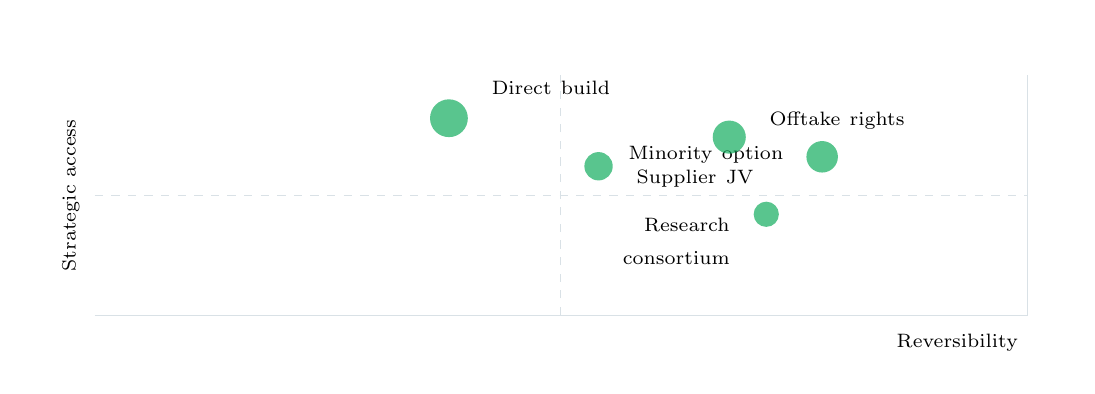
\begin{tikzpicture}[x=1cm,y=1cm]
\path[use as bounding box] (0,0) rectangle (13.20,4.30);
\draw[BOLine] (0.85,0.65) -- (12.70,0.65) -- (12.70,3.70);
\draw[BOLine,dashed] (0.85,2.17) -- (12.70,2.17);
\draw[BOLine,dashed] (6.77,0.65) -- (6.77,3.70);
\fill[BOGreen,opacity=.65] (10.09,2.66) circle (0.20);
\node[anchor=east,align=right,text width=2.10cm] at (9.72,2.69) {\scriptsize Minority option};
\fill[BOGreen,opacity=.65] (8.91,2.91) circle (0.21);
\node[anchor=west,align=left,text width=2.10cm] at (9.30,3.12) {\scriptsize Offtake rights};
\fill[BOGreen,opacity=.65] (7.25,2.54) circle (0.18);
\node[anchor=west,align=left,text width=2.10cm] at (7.61,2.38) {\scriptsize Supplier JV};
\fill[BOGreen,opacity=.65] (5.35,3.15) circle (0.24);
\node[anchor=west,align=left,text width=2.10cm] at (5.77,3.54) {\scriptsize Direct build};
\fill[BOGreen,opacity=.65] (9.38,1.93) circle (0.16);
\node[anchor=east,align=right,text width=2.10cm] at (9.04,1.59) {\scriptsize Research consortium};
\node[anchor=north east] at (12.70,0.53) {\scriptsize Reversibility};
\node[anchor=center,rotate=90] at (0.55,2.17) {\scriptsize Strategic access};
\end{tikzpicture}\par\vspace{2pt}
\vspace{1pt}\noindent\begin{minipage}[t]{0.92\linewidth}
{\footnotesize\color{BOText} Early moves should protect access and learning while avoiding positions that cannot be reversed if evidence weakens.}\par
\end{minipage}\par\vspace{1pt}
\vspace{4pt}{\footnotesize\color{BOText} Early moves should protect access and learning while avoiding positions that cannot be reversed if evidence weakens.}\par
{\scriptsize\color{BOMuted} BlueOcean competitive posture screen.}\par

\clearpage
\label{chap:8}
\noindent\begin{tikzpicture}
\path[use as bounding box] (0,0) rectangle (\linewidth,54mm);
\clip (0,0) rectangle (\linewidth,54mm);
\node[anchor=north west,inner sep=0] at (0,54mm) {
\includegraphics[width=\linewidth]{assets/image-8.png}};
\end{tikzpicture}
\vspace{0pt}
\noindent
\begin{tikzpicture}
\fill[BOGreen] (0,0) rectangle (96mm,1.2pt);
\end{tikzpicture}\par\vspace{8pt}
{\Large\sffamily\bfseries\color{BONavy} Regulation, policy and public acceptance can reset the speed of adoption}\par\vspace{4pt}
{\sffamily\fontsize{15}{20}\selectfont\color{BOGreen} External rules can accelerate the market or change the risk budget and project timeline.}\par\vspace{9pt}
\begin{multicols}{2}
{\small For leadership teams, policy support, permitting rules, standards and public acceptance affect how quickly an opportunity moves from concept to deployment. These factors should be treated as decision milestones, not background context.}\par
{\small A practical reading is that where the regulatory path is unclear, the better move is usually standards engagement, policy tracking and low-risk pilots rather than an early heavy-asset commitment.}\par
{\small The decision lens is that the board should track which policy events would change investment timing, such as licensing rules, procurement requirements, subsidy treatment, local approvals or safety standards.}\par
{\small For a CEO, Regulation, policy and public acceptance can reset the speed of adoption matters only if it changes the timing of capital, partner access, customer commitments or risk appetite. The strongest posture is to keep learning close to the business while reserving heavier commitments for proof that can survive investment-committee scrutiny.}\par
{\small For Regulation, policy and public acceptance can reset the speed of adoption, resource allocation should follow the facts that can change the decision: customer demand, cost position, financing availability, regulatory path and delivery capability. If those facts do not improve, increasing exposure mainly creates strategic lock-in rather than higher conviction.}\par
\end{multicols}
\label{chap:8:end}

\clearpage
{\sffamily\fontsize{20}{25}\selectfont\color{BONavy} About the research}\par\vspace{6pt}
\vspace{2pt}{\color{BOBright}\rule{\linewidth}{1pt}}\vspace{5pt}
{\footnotesize\color{BOMuted} This report has been prepared for strategy discussion and executive decision support. It is not investment, legal, tax, audit or valuation advice. Market estimates, forecasts and scenarios are directional and should be independently validated before they are used for investment, financing, transaction, regulatory or operational decisions. Forward-looking views may change as technology, policy, financing, regulation, competition, supply chains and macro conditions evolve. Recipients should perform their own diligence and treat this report as one input into a broader decision process.}


\clearpage
\thispagestyle{empty}
\begin{tikzpicture}[remember picture,overlay]
\node[anchor=south west,inner sep=0] at (current page.south west) {
\includegraphics[width=\paperwidth,height=\paperheight]{assets/cover-ai.png}};
\fill[black,opacity=.45] (current page.south west) rectangle (current page.north east);
\node[anchor=south east] at ([xshift=-11mm,yshift=10mm]current page.south east) {\sffamily\bfseries\Large\color{white} BlueOcean};
\end{tikzpicture}

\end{document}
